\Lecturer{Hui Jin}
\Contributor{}
\LectureNumber{13}
\LectureDate{DATE}
\LectureTitle{Introduction to Quantum Information}

\lstset{style=mystyle}


	\MakeScribeTop

%#############################################################
%#############################################################
%#############################################################
%#############################################################

\section{Introduction}
[J Preskill] In quantum theory, the act of acquiring information about a physical system inevitably disturbs the state of the system. There is no counterpart of this limitation in classical physics.

That acquiring information causes a disturbance is also connected with another essential distinction between quantum and classical information: quantum information cannot be copied with perfect fidelity. If we could make a perfect copy of a quantum state, we could measure an observable of the copy without disturbing the original and we could defeat the principle of disturbance. On the other hand, nothing prevents us from copying classical information perfectly.

These properties of quantum information are important, but the really deep way in which quantum information differs from classical information emerged from the work of John Bell. Bell showed that quantum information can be (in fact, typically is) encoded in nonlocal correlations between the different parts of a physical system, correlations with no classical counterpart. 

The study of quantum information as a coherent discipline began to emerge in the 1980’s, and it has blossomed in the 1990’s.

\section{The Qubit}
The unit of classical information is the bit, which can take either one of two values: \(0\) or \(1\). The corresponding unit of quantum information is the quantum bit or qubit. The qubit is a vector in a two dimensional complex vector space with inner product (A Hilbert Space of dimension of \(2\)). We can call the elements of an orthonormal basis in this space \(\ket{0}\) and \(\ket{1}\), by using the Dirac's ket notation. Conventionally, the orthonormal basis \(\ket{0}\) and \(\ket{1}\) are taken to be
\begin{align*}
    \ket{0} = \begin{bmatrix}
           1 \\
           0 
         \end{bmatrix}
    , \;\;\;
    \ket{1} = \begin{bmatrix}
           0 \\
           1 
         \end{bmatrix}.
  \end{align*}
  
  Then a normalized vector can be represented
\[\ket{\psi} = \alpha \ket{0} + \beta \ket{1} =  \begin{bmatrix}
           \alpha \\
           \beta 
    \end{bmatrix},
\] 
where \(\alpha, \beta \in C\) and \(|\alpha|^2 + |\beta|^2 = 1\). This defines a qubit, a superposition of the two base vectors. We can perform a measurement that projects \(\ket{\phi}\) onto the basis \(\ket{0}\), \(\ket{1}\). The outcome of the measurement is not deterministic — the probability that we obtain the result \(\ket{0}\) is \(|\alpha|^2\) and the probability that we obtain the result \(\ket{1}\) is \(|\beta|^2\). Once measured, superposition of the qubit is removed and the qubit collapsed to the classical bit. 

Nature operates in the quantum world, and stores information in a superposition way. The most revealing observation is the double slit experiment. 

Two important superposition states are
\[\frac{1}{\sqrt{2}}(\ket{0} +\ket{1}) \]
and
\[\frac{1}{\sqrt{2}}(\ket{0} - \ket{1}) \]
These will come up repeatedly. They are often referred to as the "\(\ket{+}\)" and "\(\ket{-}\)" states, for obvious reasons. If \(\ket{0}\) and \(\ket{1}\) are vectors pointing along the \(x\) and \(y\) axes, then \(\ket{+}\) and \(\ket{-}\) are the diagonal vectors. Note that \(\ket{+}\) and \(\ket{-}\) are orthogonal to one another and act in all respects like an alternative pair of basis states. 

\subsection{Exponential Dimension of \(n\)-qubits}
We know \(N\) classical bits can take \(2^N\) possible values; the system of \(N\) classical bits has dimension of \(N\) as we can use a binary string of length \(N\) to describe it. A configuration of \(N\) qubits, on the other hand, requires \(2^N\) complex numbers for a complete description. Therefore the dimension of N-qubits is \(2^N\), growing exponentially with the number of qubits.   

For instance, to describe a configuration of \(100\) classical bits, we need \(100\) bits; to describe a configuration of \(100\) qubits in the classical world, we need \(2^{100}\) complex numbers. Here lies the difficulty of using classical computation systems to simulate a quantum world.

\subsection{Multiple Qubits Tensor Product}
The tensor product (or Kronecker product) is used to combine quantum states. The combined state for a qubit register is the tensor product of the constituent qubits. The tensor product is denoted by the symbol 
\(\otimes\).
The vector representation of two qubits is:
\[
\ket{\psi} = v_{00}\ket{00} + v_{01}\ket{01} + v_{10}\ket{10} + v_{11}\ket{11}
\rightarrow {\begin{bmatrix}v_{00}\\v_{01}\\v_{10}\\v_{11}\end{bmatrix}}.
\]

\section{Linearity of Quantum Mechanics}
The linearity of quantum mechanics (QM) is a fundamental feature. This linearity does not depend on the particular object under study, provided it is sufficiently isolated from anything else. It is naturally reflected in the superposition principle and entails the “quantum essentials” interference and entanglement, without which modern applications of QM, e.g. in precision measurement and information technologies, and the ongoing study of the foundations of QM would not be the same.

In our discussion, we assume all manipulation of the qubits are through unitary operations, which are linear. Thus we can analyze a quantum circuit first using the base vectors, and then for the general qubits, the effect can be obtained by superposition principle. This approach is fundamental in our analysis. 

\section{The Quantum Logic Gates}
In quantum computing and specifically the quantum circuit model of computation, a quantum logic gate (or simply quantum gate) is a basic quantum circuit operating on a small number of qubits. Quantum logic gates are the building blocks of quantum circuits, like classical logic gates are for conventional digital circuits.

Quantum gates are unitary operators, and can be described unitary matrices. In the following, we describe the building blocks of these quantum gates.

A gate that acts on \(n\) qubits is represented by a \(2^n \times 2^n\) unitary matrix. 

\subsection{Quantum gates on one-qubit}
The Pauli matrices are a set of three \(2 \times 2\) complex matrices that are Hermitian and unitary. We manipulate qubits by applying Pauli matrices; they are also how the environment introduces noise onto the qubits. 

\paragraph{X} 
Pauli Matrix \(X\) swaps the base states:
\begin{align*}
    X \ket{0} &= \ket{1} \\
    X \ket{1} &= \ket{0} 
\end{align*}
Based on such transformation, we know that 
$$X = \begin{bmatrix}
    0 & 1 \\
    1 & 0 
\end{bmatrix}$$

By linearity of quantum states, we have for a general qubit \(\ket{q}\), 
\begin{align*}
    X \ket{q} = X (\alpha \ket{0} + \beta \ket{1}) &= \alpha \ket{1} + \beta \ket{0}
\end{align*}
Equivalently, this can be represented by the unitary matrix operation \(X\begin{bmatrix}
           \alpha \\
           \beta 
    \end{bmatrix} = \begin{bmatrix}
           \beta \\
           \alpha 
    \end{bmatrix} 
    \).
\paragraph{Z} 
Pauli Matrix \(Z\) introduces a phase shift to the qubit:
\begin{align*}
    Z \ket{0} &= \ket{0} \\
    Z \ket{1} &= -\ket{1} \\
    Z (\alpha \ket{0} + \beta \ket{1}) &= \alpha \ket{0} - \beta \ket{1}
\end{align*}
Based on such transformation, we know that 
$$Z = \begin{bmatrix}
    1 & 0 \\
    0 & -1 
\end{bmatrix}$$

\paragraph{Y} Pauli matrix \(Y\) introduces a bit flip and a phase shift to a qubit: 
\begin{align*}
    Y \ket{0} &= i\ket{1} \\
    Y \ket{1} &= -i\ket{0} \\
    Y (\alpha \ket{0} + \beta \ket{1}) &= i(\alpha \ket{1} - \beta \ket{1})
\end{align*}
Based on such transformation, we know that 
$$Y = \begin{bmatrix}
    0 & -i \\
    i & 0 
\end{bmatrix}$$

The Pauli matrices are involutory, meaning that the square of a Pauli matrix is the identity matrix.
 \[X^2 = Y^2 = Z^2 = -iXYZ = I\] and \[ZX=-XZ = iY\]. 

\paragraph{Hadamard Matrix H} 
The Hadamard matrix \(H\) maps one normalized basis to another normalized basis: 
\begin{align*}
    H \ket{0} &= \frac{1}{\sqrt{2}}( \ket{0} + \ket{1}) = \ket{+} \\
    H \ket{1} &= \frac{1}{\sqrt{2}}( \ket{0} - \ket{1}) = \ket{-} \\
    H (\alpha \ket{0} + \beta \ket{1}) &= \alpha \ket{+} + \beta \ket{-}
\end{align*}
Based on such transformation, we know that 
$$H = \frac{1}{\sqrt{2}}\begin{bmatrix}
    1 & 1 \\
    1 & -1 
\end{bmatrix}$$


\subsection{Quantum gates on multi-qubits}
\paragraph{CNOT Gate}
The controlled NOT gate (or CNOT or CX) acts on 2 qubits, and performs the NOT operation on the second qubit only when the first qubit is \(\ket{1}\), and otherwise leaves it unchanged. With the convention of using the left qubit \(\ket{b_1}\) as the control bit in \(\ket{b_1b_2}\), we have

\begin{align*}
    CX \ket{00} &= \ket{00} \\
    CX \ket{01} &= \ket{01} \\
    CX \ket{10} &= \ket{11} \\
    CX \ket{11} &= \ket{10} 
\end{align*}

 Based on such transformation, we know that it is represented by the Hermitian unitary matrix:
$$CX = \begin{bmatrix}
    1 & 0 & 0 & 0  \\
    0 & 1 & 0 & 0  \\
    0 & 0 & 0 & 1  \\
    0 & 0 & 1 & 0   
\end{bmatrix}$$

The quantum circuit of the CNOT gate is depicted in Figure~\ref{fig:cnot}
\begin{figure}[h]
    \centering
    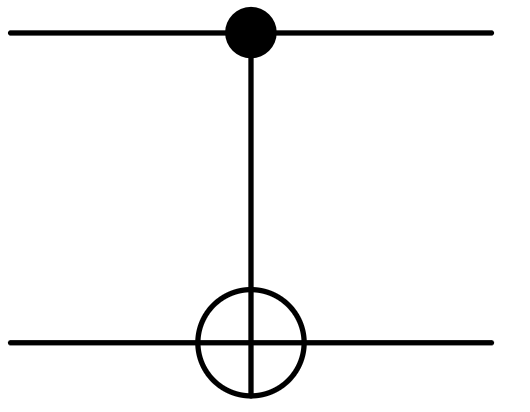
\includegraphics[width=0.3\textwidth]{Figs/cnot.png}
    \caption{CNOT gate performs the NOT operation on the second qubit only when the first qubit is \(\ket{1}\), and otherwise leaves it unchanged. }
    \label{fig:cnot}
\end{figure}


\paragraph{SWAP Gate}
The swap gate (SWAP) performs the swap operation on the two qubits; we have

\begin{align*}
    SWAP \ket{00} &= \ket{00} \\
    SWAP \ket{01} &= \ket{10} \\
    SWAP \ket{10} &= \ket{01} \\
    SWAP \ket{11} &= \ket{11} 
\end{align*}
Based on such transformation, we know that it is represented by the Hermitian unitary matrix:
$$CX = \begin{bmatrix}
    1 & 0 & 0 & 0  \\
    0 & 0 & 1 & 0  \\
    0 & 1 & 0 & 0  \\
    0 & 0 & 0 & 1   
\end{bmatrix}$$

The quantum circuit of the SWAP gate is depicted in Figure~\ref{fig:swap}
\begin{figure}[h]
    \centering
    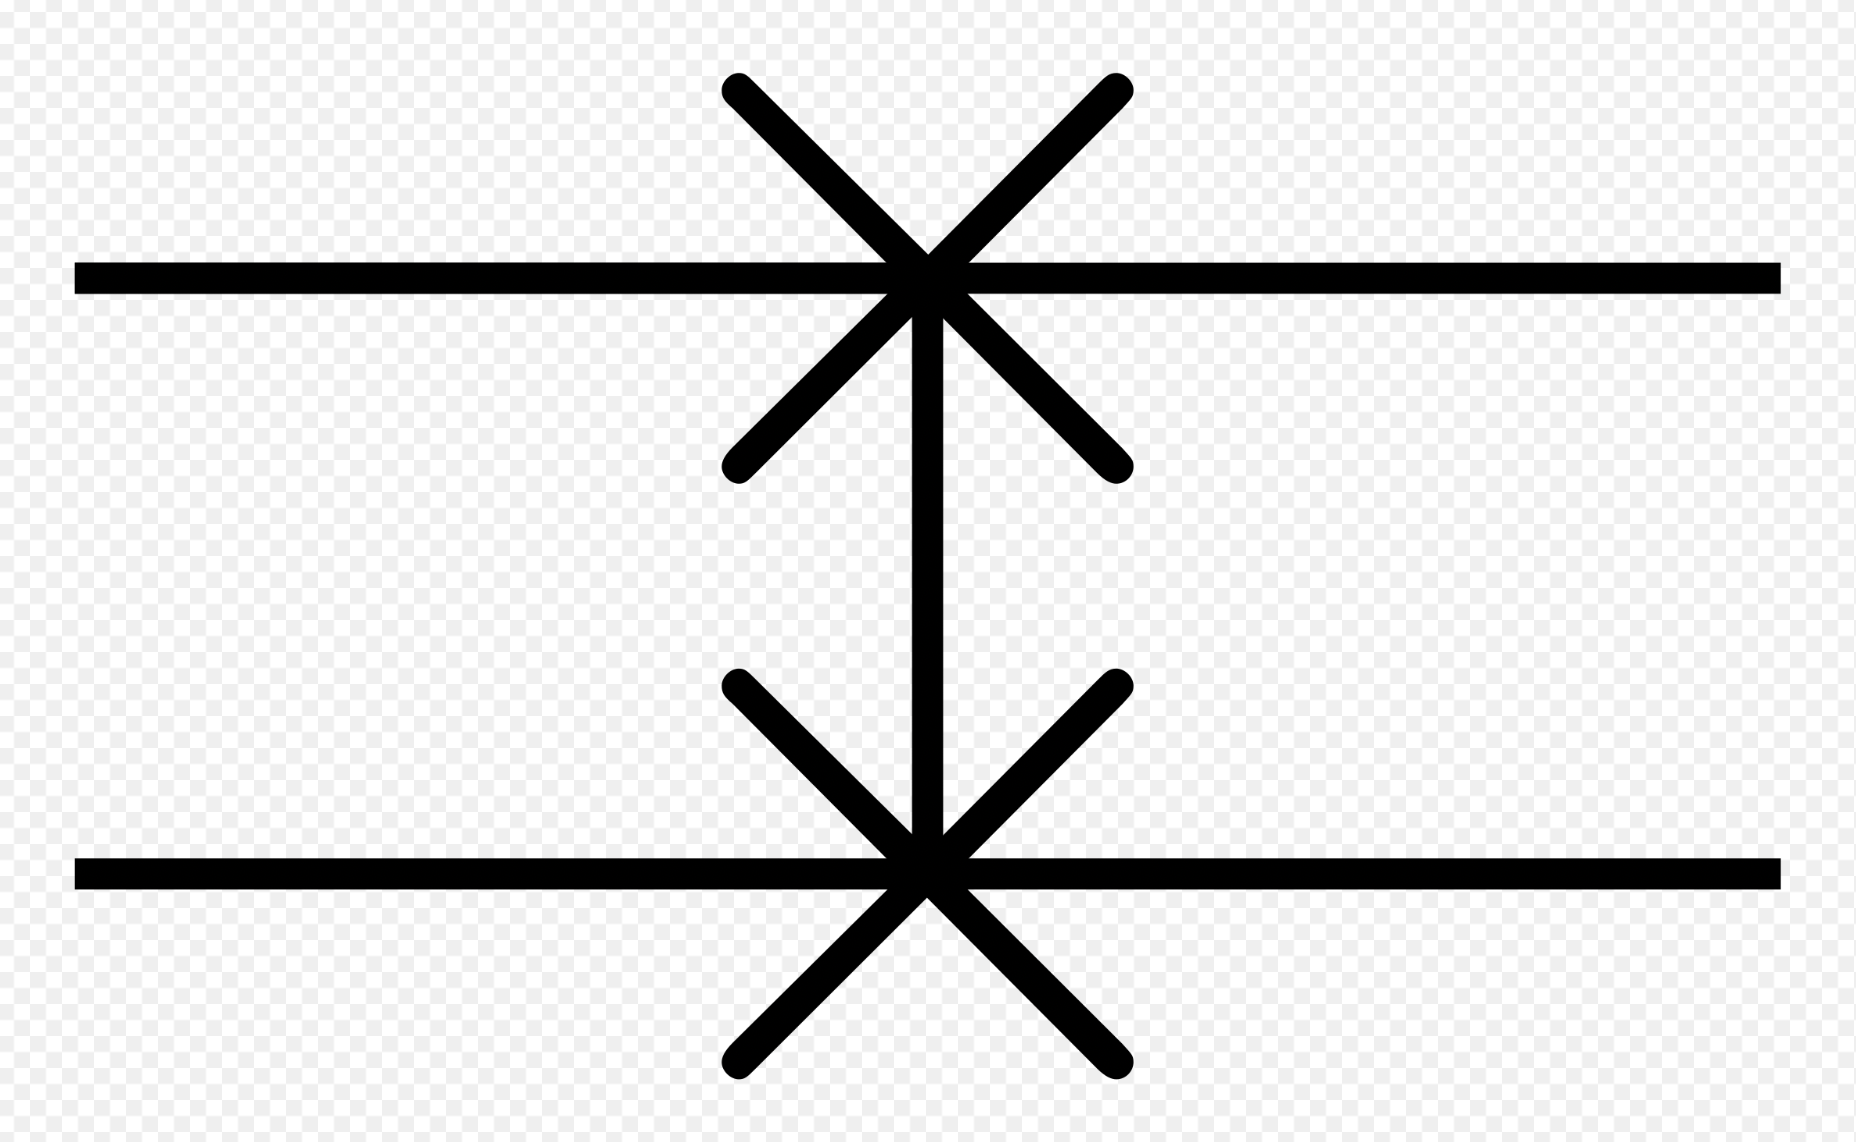
\includegraphics[width=0.3\textwidth]{Figs/swap.png}
    \caption{SWAP gate performs the swap of the two qubits. }
    \label{fig:swap}
\end{figure}


\paragraph{Toffoli Gate}
The quantum Toffoli gate is defined for \(3\) qubits. It is an extension of the CNOT gate; it performs the NOT operation on the third qubit if and only if the first two qubits are both \(\ket{1}\).

We have
\begin{align*}
    TOFF \ket{110} &= \ket{111} \\
    TOFF \ket{111} &= \ket{110} \\
    TOFF \ket{abc} &= \ket{abc} \; \; \text{all other three qubits}
\end{align*}

The quantum circuit of the Toffoli gate is depicted in Figure~\ref{fig:tofolli}
\begin{figure}[h]
    \centering
    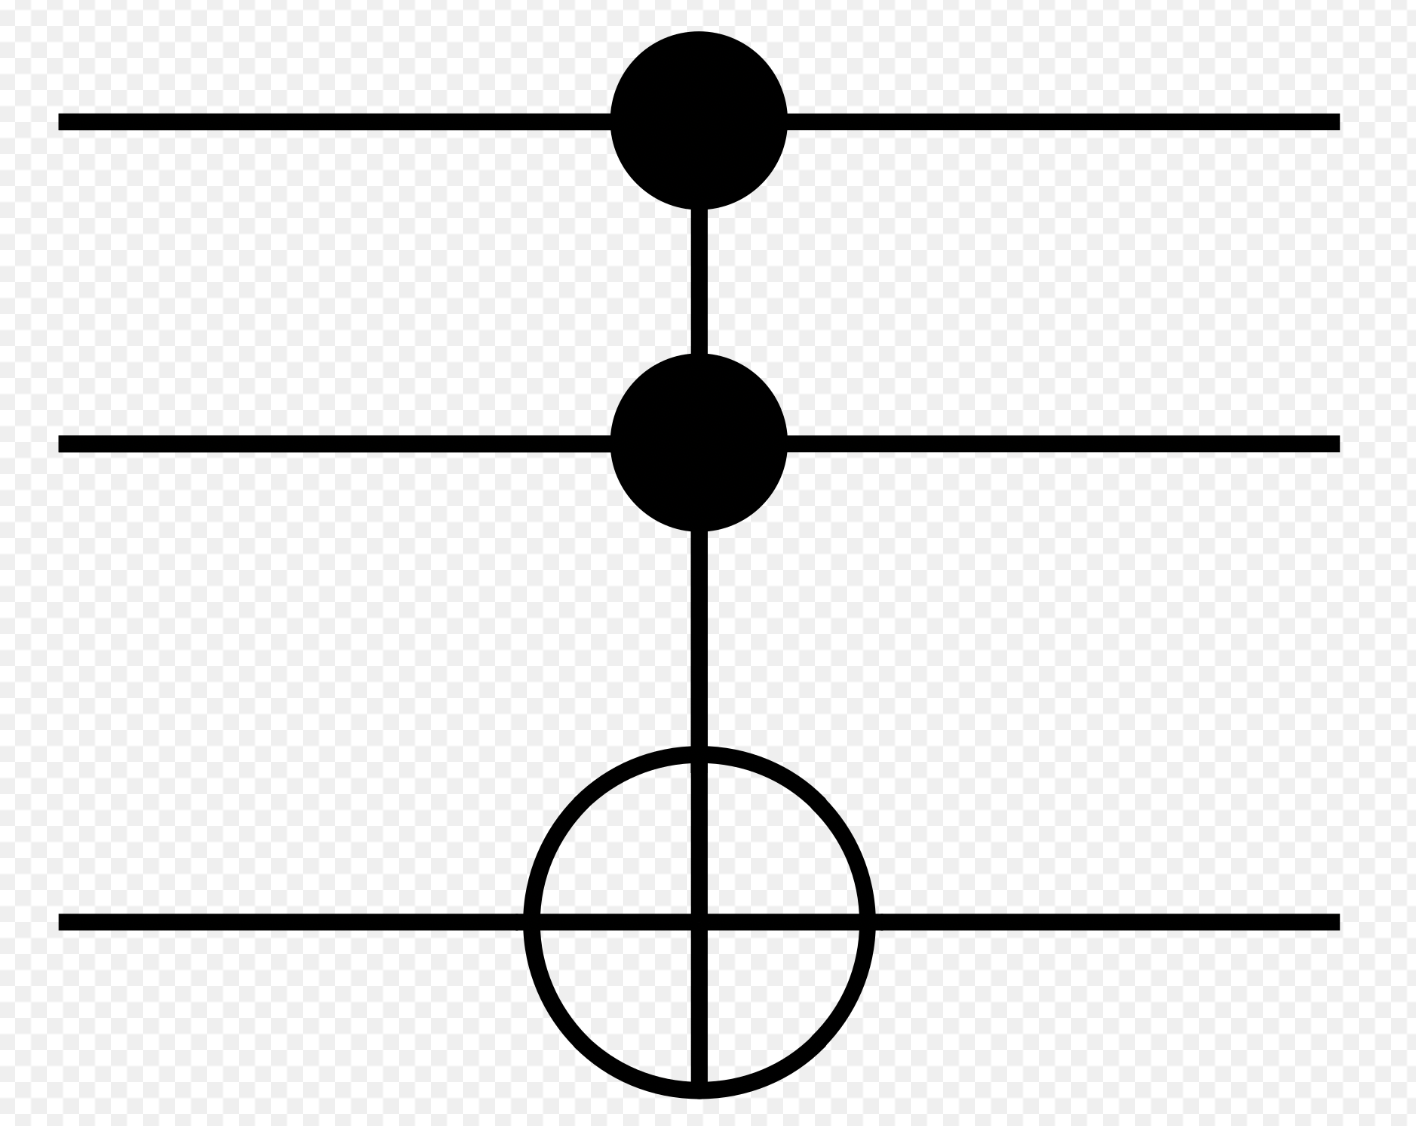
\includegraphics[width=0.3\textwidth]{Figs/Toffoli.png}
    \caption{Toffoli gate performs NOT operation on the third bit if and only both the first two qubits are \(\ket{1}\). }
    \label{fig:tofolli}
\end{figure}

\section{The standard ways to analyze a quantum circuit}
To analyze the output state of a quantum circuit, there are some standard approaches. 

The first common approach rests on the linear property of quantum circuit. If we know the output for every basis state, we know the operation matrix as each basis state corresponds to a column of the operation matrix. If fact, that is the basic approach for us to obtain the unitary matrix representation for the basic quantum gates. 

The second common approach is more for complicated circuits. With a concatenation of simple circuits, sometimes it is simpler to use the matrix multiplication to analyze the circuit.


\paragraph{break here}

\section{Some important quantum circuits}

\subsection{Repetition Circuit}
An important technique in classical coding is to use repetition. We can achieve a similar repetition using entanglement. 

It is easy to check in the CNOT gate, if we let the control qubit be \(\ket{x}\) and the second qubit be \(\ket{0}\), then the output qubits is \(\ket{xx}\). 


If the inputs are superposition: \(\alpha\ket{0}+ \beta\ket{1}\), then the quantum circuit will produce  
\[\alpha\ket{00} + \beta\ket{11}.\]

\begin{figure}[h]
    \centering
    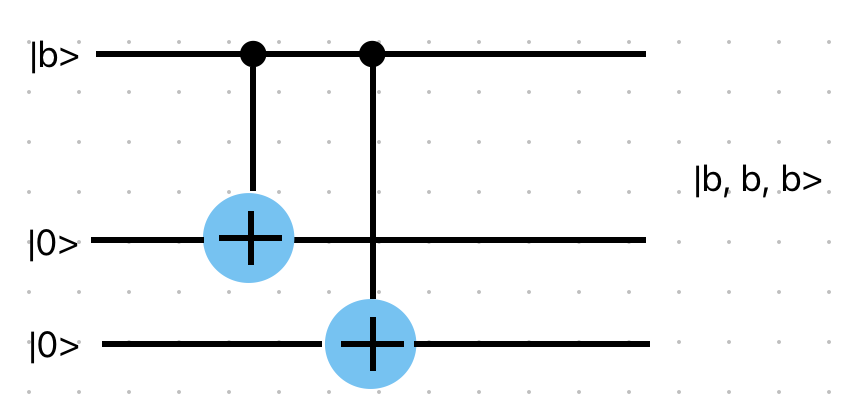
\includegraphics[width=0.6\textwidth]{Figs/QEC_Repeat.png}
    \caption{Qubit repetition through entanglement.}
    \label{fig:QEC_repeat}
\end{figure}

We can use the same control bit \(\ket{x}\) to control another NOT gate on another qubit \(\ket{0}\), like in Figure~\ref{fig:QEC_repeat} and produce another repeated qubit and the resulted output will be 
\[\alpha\ket{000} + \beta\ket{111}.\]


\subsection{Parity check circuit}
An important technique in classical coding is to use parity check bits. We can achieve a similar parity check qubits using entanglement. 

For example, Figure~\ref{fig:QECParity} shows the quantum circuit that takes in two base (\(\ket{0}\) or \(\ket{1}\)) qubits \(\ket{x}\) and \(\ket{y}\) and generate at the output entangled state \(\ket{x, y, x+y}\)

\begin{figure}[h]
    \centering
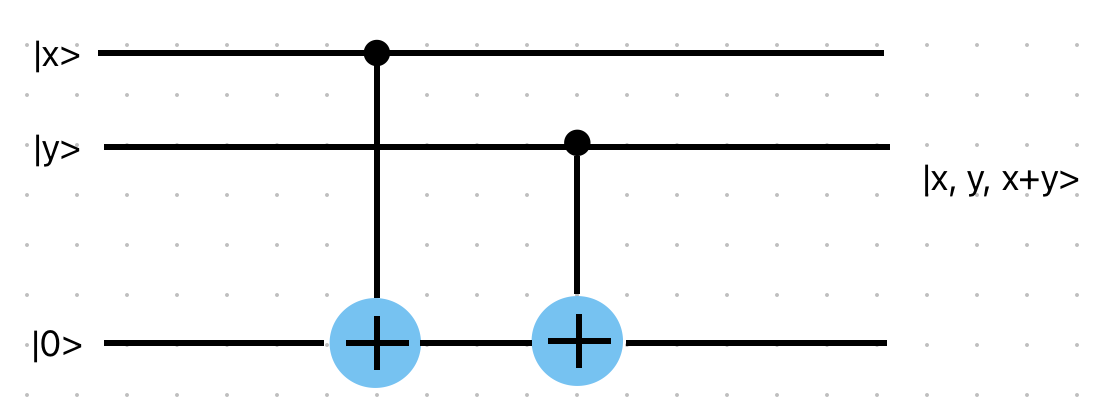
\includegraphics[width=0.75\textwidth]{Figs/QecParityCheck.png}
    \caption{Quantum circuit to parity check qubits through entanglement}
    \label{fig:QECParity}
\end{figure}

What if the inputs are superposition of \(\ket{0}\) and \(\ket{1}\), for example \(\ket{x} = \ket{y} = \ket{+}\), then the quantum circuit will produce at the output, by considering the base states, 
\[\frac{1}{2}(\ket{000} + \ket{011} + \ket{101} + \ket{110}).\]
As we see, in each of the base states generated, the binary representation of the qubits satisfies the parity check.

\subsection{The action of Hadamard Transformation}
We know that \(H\ket{0} = \frac{1}{2}\ket{+}\) and  \(H\ket{1} = \frac{1}{2}\ket{-}\). If we do Hadamard transformation to n-qubits in parallel, we can generate a uniform distribution on all possible \(n\)-bit base states. First, the transformed result on the all zero base vector is easy to see: 
\begin{lemma}
The action of \(H^{n}\) on n-qubit \(\ket{0^n}\) yields the transformation
\begin{align*}
H^{n}\ket{0^n} = \frac{1}{\sqrt{2^n}} \sum_{z=0}^{2^n-1} \ket{z}  
\end{align*}
\end{lemma}
\begin{proof}
\end{proof}


This result can be generalized to the transformation on any base vector: 
\begin{lemma}
The action of \(H^{n}\) on any n-qubit \(\ket{x}\) yields the transformation
\begin{align*}
H^{n}\ket{x} = \frac{1}{\sqrt{2^n}} \sum_{z} (-1)^{x\cdot z} \ket{z}     
\end{align*}

where \(z\) enumerates all possible \(n\)-bit combination and \(x\cdot z\) is a bit-wise dot-product. 
\label{lemma:HadamardAction}    
\end{lemma}

\begin{proof}
    We prove this by induction. 
\end{proof}

\subsection{Bell's States}
 We consider Hadamard gate and a CNOT gate as in Figure~\ref{fig:bell00}. Different combination of inputs will generate the four Bell's states. For example, in the figure the quantum circuit takes the two qubit input \(\ket{00}\) and transforms it to the first Bell state \(\ket{\phi^{+}}\). Explicitly, the Hadamard gate transforms \(\ket{00}\) into a superposition of \(\ket{+}\ket{0}\). This will then act as a control input to the CNOT gate, which only inverts the target (the second qubit) when the control (the first qubit) is \(1\). Thus, the CNOT gate transforms the second qubit as follows 
\(\frac {1}{\sqrt{2}}(\ket{00} + \ket{11})\).

\begin{figure}[h]
    \centering
    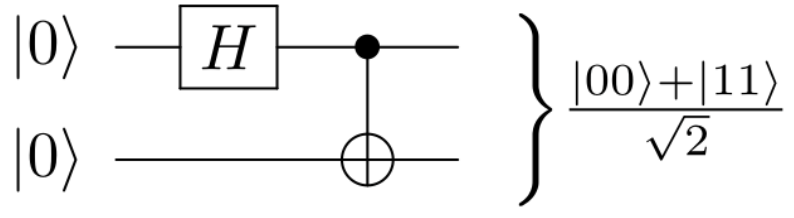
\includegraphics[width=0.5\textwidth]{Figs/BellState00.png}
    \caption{Quantum circuit to generate Bell state}
    \label{fig:bell00}
\end{figure}
Input \(\ket{10}\) will generate \(\ket{\phi^{-}}\) and so on.

 The Bell's states or EPR pairs are specific quantum states of two qubits that represent the simplest examples of quantum entanglement, a property that is essential in quantum computation. 




\section{The Magic of Quantum Algorithms}
The exciting new result that Shor found is that a quantum computer can factor in polynomial time, e.g., in time \(O(\ln n)^3\).

 design of quantum algorithms that solve certain problems faster than classical algorithms can.

Quantum algorithm is not for every problem.

This is possible because the quantum computer is not limited to computing either \(f(0)\) or \(f(1)\). It can act on a superposition of \(\ket{0}\) and \(\ket{1}\), and thereby extract “global” information about the function, information that depends on both \(f(0)\) and \(f(1)\). This is quantum parallelism.

Our exploration of quantum algorithms shall begin with the solution of a very basic problem: finding whether or not a Boolean function \(f(x)\) is a constant. The solution is given by the Deutsch algorithm, which illustrates a fundamental property of quantum computing, namely parallelism. As we shall indeed see, quantum computation makes it possible to evaluate \(f(x)\) simultaneously for all values of the variable \(x\), in contrast to classical computing where such an evaluation must be performed one variable at a time, or through as many computers working in parallel.

\subsection{The Deutsch Algorithm}
The problem Deutsch’s algorithm tackles can now be stated as follows. Given a block box Uf implementing some unknown function \(f : \{0,1\} \rightarrow \{0,1\},\) determine whether \(f\) is “constant” or “balanced”. Here, constant means \(f\) always outputs the same bit, i.e. \(f(0) = f(1)\), and balanced means f outputs different bits on different inputs, i.e. \(f(0)  \neq f(1)\).

\paragraph{Oracle} We are given a function oracle as depicted in Figure~\ref{fig:Uf}. The oracle is expensive to use, so we want to use as few times as possible. 

\begin{figure}[h]
    \centering
    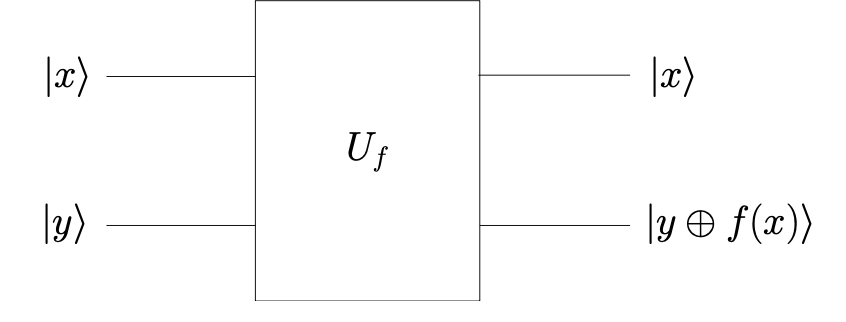
\includegraphics[width=0.5\textwidth]{Figs/FunctionOracle.png}
    \caption{Quantum circuit of a unitary operator mapping \(\ket{x}\ket{y} \rightarrow \ket{x}\ket{y\oplus f(x)}\) for any \(x, y \in \{0, 1\}\) (i.e. \(\ket{x}, \ket{y}\) denote standard basis states)}
    \label{fig:Uf}
\end{figure}

Observe now that \(U_f\) is reversible — this is because running \(U_f\) again on its output returns the original state \(\ket{x}\ket{y}\). Also note that we have not specified the inner workings of \(U_f\) but will rather treat \(U_f\) as a “black box” or “oracle” which we presume we can run, but cannot “look inside” to see its implementation details.

Of course, there is an easy way to determine whether f is constant or balanced — simply evaluate f on inputs 0 and 1, i.e. compute f(0) and f(1), and then check if f(0) = f(1). This naive (classical) solution, however, requires two queries or calls to \(U_f\) (i.e. one to compute \(f(0)\) and one to compute \(f(1)\)). So certainly at most two queries to Uf suffice to solve this problem. Can we do it with just one query? Classically, the answer turns out to be no. But quantumly, Deutsch showed how to indeed achieve this with a single query.

\begin{figure}[h]
    \centering
    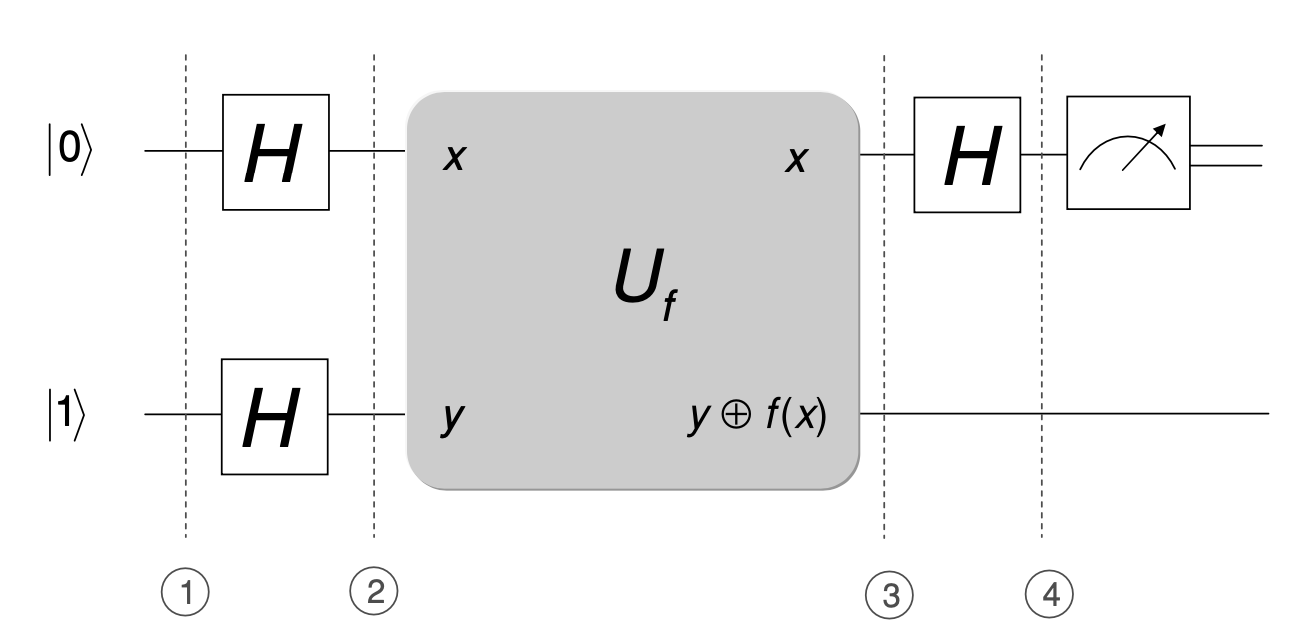
\includegraphics[width=0.7\textwidth]{Figs/DeutschCircuit.png}
    \caption{The Deutsch Algorithm}
    \label{fig:Deutsch}
\end{figure}

Let us walk through the steps: 
\begin{align*}
    \ket{\psi_1} &= \ket{0}\ket{1} \\
    \ket{\psi_2} &= \ket{+}\ket{-} = \frac{1}{\sqrt{2^2}}(\ket{0} + \ket{1})(\ket{0} - \ket{1}) = \frac{1}{\sqrt{2^2}}(\ket{0}(\ket{0} - \ket{1}) + \ket{1}(\ket{0} - \ket{1}))\\
    \ket{\psi_3} &= \frac{1}{\sqrt{2^2}}(\: \ket{0}(\ket{0\oplus f(0)} - \ket{1\oplus f(0)}) + \ket{1}(\ket{0\oplus f(1)} - \ket{1\oplus f(1)}) \:) \\
           &= \frac{1}{\sqrt{2^2}}(\:\ket{0}(-1)^{f(0)}(\ket{0} - \ket{1}) + \ket{1}(-1)^{f(1)}(\ket{0} - \ket{1})\:) \\
           &= \frac{1}{\sqrt{2}}(\:\ket{0}(-1)^{f(0)} + \ket{1}(-1)^{f(1)}\:) \ket{-} \\    
\end{align*}
At this step, we can drop the second qubit and focus on the first qubit. Transform this qubit by a Hadamard matrix, we have
\begin{align*}
 \ket{\psi_4} &= \frac{1}{2} ((-1)^{f(0)} \ket{+} + (-1)^{f(1)} \ket{-}) \\
        &= \frac{1}{2} ( (-1)^{f(0)} +
(-1)^{f(1)})\ket{0} +  ((-1)^{f(0)} -
(-1)^{f(1)})\ket{1} ) \\  
\end{align*}
The measurement, by projecting onto the basis \(\{\ket{0}, \ket{1}\) will either be in classical state \(0\) when \(f(0) = f(1)\)  or \(1\) when \(f(0) \neq f(1).\) 
 
\subsection{The Deutsch-Jozsa Algorithm}
The Deutsch-Jozsa algorithm is the generalization of the Deutsch algorithm: it determines whether a function \(f: \{0,1\}^n \rightarrow \{0,1\}\) is constant or balanced if it is promised only these two are the only possibilities. 

It will be a great exercise to walk through the qubits in the Figure~\ref{fig:DeutschJozsa}. 

\begin{align*}
    \ket{\psi_0} &= \ket{0}^{\otimes n}\ket{1} \\
    \ket{\psi_1} &= \frac{1}{\sqrt{2^n}}\ket{+}^{\otimes n}\ket{-} \\
           &= \frac{1}{\sqrt{2^n}} \sum_{x=0}^{2^n-1} \ket{x}\ket{-} \\
    \ket{\psi_2} &= \frac{1}{\sqrt{2^{n+1}}}\sum_{x=0}^{2^n-1}\ket{x} (\ket{0\oplus f(x)} - \ket{1\oplus f(x)} \\
           &= \frac{1}{\sqrt{2^{n+1}}}\sum_{x=0}^{2^n-1}\ket{x}(-1)^{f(x)} (\ket{0} - \ket{1}) \\
           &= \frac{1}{\sqrt{2^{n}}}\sum_{x=0}^{2^n-1}\ket{x}(-1)^{f(x)} \ket{-} \\ 
\end{align*}

\begin{figure}[h]
    \centering
    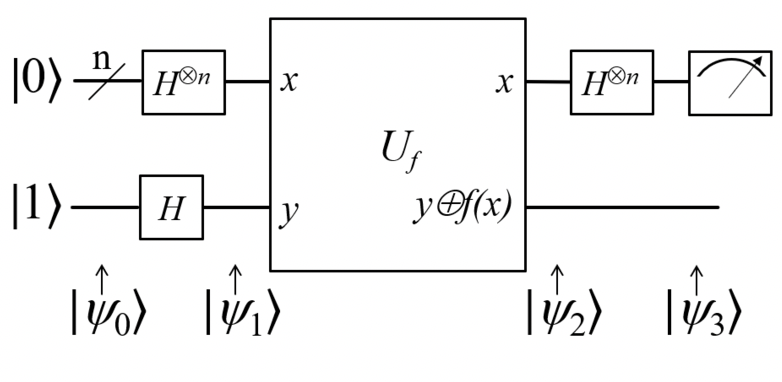
\includegraphics[width=0.7\textwidth]{Figs/Deutsch_algorithm.png}
    \caption{The Deutsch-Jozsa Algorithm}
    \label{fig:DeutschJozsa}
\end{figure}

At this stage, we can drop the last qubit and focus on the first \(n\) qubits. Transform them by a Hadamard matrix, by Lemma 6.2, we have
\begin{align*}
 \ket{\psi_3} &= \frac{1}{2^n} \sum_{x=0}^{2^n-1} \sum_{x} (-1)^{f(x)} \sum_z (-1)^{x\cdot z} \ket{z}  \\  
 &= \frac{1}{2^n} \sum_z  \ket{z} \sum_{x} (-1)^{f(x) + x \cdot z} \\
\end{align*}

If we focus on the \(\ket{z=0}\) state, its coefficient is  \(\frac{1}{2^n}(\sum_{x} (-1)^{f(x)})\), which is either \(1\) if \(f(x)\) is constant or \(0\) if \(f(x)\) is balanced. In the first case, this must be the only quantum state the system is in as the quantum state has coefficient. Projecting onto this state thus gives us the computational desired result whether the function is balanced or constant.  

\section{Exercise}
p1. Calculate the output quantum state of the following circuit if the input \(x_1 = \ket{0}, x_2 = \ket{0}\).

\begin{figure}[h]
    \centering
    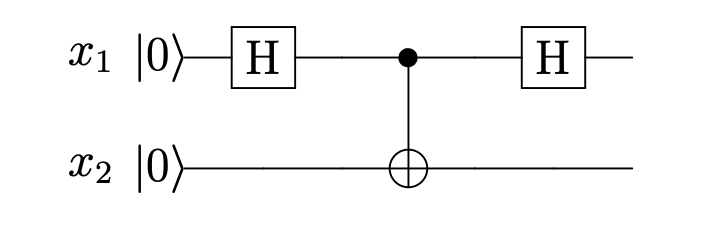
\includegraphics[width=0.5\textwidth]{Figs/QI_p1.png}
    \caption{Quantum circuit to analyze}
    \label{fig:QIex1}
\end{figure}


p2. A SWAP gate takes two inputs \(x_1\) and \(x_2\) and outputs \(x_2\) and \(x_1\); i.e., it swaps the values of two registers. Show how to build a SWAP gate using only CNOT gates. (Hint: you’ll need \(3\) of them.)